\chapter{Metamodel}
Durch das Metamodel wird eine Beschreibung vorgegeben, mit der man die einzelnen Module der Basissoftware und Sofwarekomponenten konfigurieren kann. Aus dieser Konfiguration lässt sich der C-Code für die RTE Schnittstellen und die Vorlagen für die Task (SWC) automatisch generieren. 
\section{Vorbereitung}
Für die Bearbeitung des Metamodels und Generierung des C-Codes benötigt man das Programm \frqq{}Eclipse Modeling Tools\flqq{} (Photon Version von Juni 2018). Bevor man starten kann, muss das Metamodell und der Generator in Eclipse hinzugefügt werden. Das Metamodell befindet sich im Ordner \frqq{}metamodel\flqq{} und der Generator im Ordner \frqq{}generators\flqq{}.
\subsection{Einstellungen im Generator}
Bevor Quellcode generiert werden kann, muss zum einem der Pfad zur *.xml Datei angegeben werden. Dies ist im Projektordner \frqq{}generators\flqq{} unter \frqq{}src/(default package)/Test.java\flqq{} in Zeile 8 einstellbar. Außerdem muss der Ordner für die Code-Ausgabe angegeben werden. Dies ist im Projektordner \frqq{}generators\flqq{} unter \frqq{}src/generator.brick/MainGenerator.java\flqq{} in Zeile 20 möglich. Im Zielordner muss nach der Generierung des C-Codes der statische BSW Code, sowie die Runnables hinzugefügt werden. Außerdem muss das jeweilige Makefile hinzugefügt werden und gegenbenenfalls der \frqq{}TARGET\_NAME\flqq{} angepasst werden.
%res Ordner in den Eigenschaften hinzufügen, Rechtsklick auf generators Project -> Properties -> Java Build Path Add folder generators/res

\section{Konfiguration des AUTOSAR Systems}
Hier eine kurze Beschreibung, wie es möglich ist, ein AUTOSAR System aus unseren Metamodel zu konfigurieren. Um eine Konfiguration zu erstellen muss zunächst eine neues AutosarMetaModel Model mit dem Model Object \frqq{}Autosar System\flqq{} erstellt werden.
\subsection{Autosar System}
Dieses Objekt ist das Root Objekt.
\paragraph{Parameter}
\begin{itemize}
\item Name
\end{itemize}
\paragraph{Kindobjekte}
\begin{itemize}
\item SWC
\item Brick
\item Connection
\end{itemize}

\subsection{SWC}
Dieses Objekt repräsentiert die Softwarekomponente. Es wird in der Konfiguration unter einem \frqq{}Autosar System\flqq{}  Objekt erstellt und  wird im \frqq{}Brick\flqq{} Objekt referenziert.
\paragraph{Parameter}
\begin{itemize}
\item Name
\end{itemize}
\paragraph{Kindobjekte}
\begin{itemize}
\item Runnables
\item ECUPorts
\item SoftwarePorts
\end{itemize}

\subsection{Brick}
Dieses Objekt repräsentiert einen NXT Hardware Brick und wird in der Konfiguration unter einem \frqq{}Autosar System\flqq{} Objekt erstellt. In diesem Objekt müssen in den Eigenschaften die \frqq{}SWC\flqq{} Objekte referenziert werden, die auf diesem Brick ausgeführt werden sollen.
\paragraph{Parameter}
\begin{itemize}
\item Bluetooth MAC
\item Bluetooth Mode
\item Name
\item Swc
\end{itemize}
\paragraph{Kindobjekte}
\begin{itemize}
\item HardwareConnection
\end{itemize}


\subsection{Connection}
Dieses Objekt ist für die Verbindung von zwei SWCs gedacht und wird in der Konfiguration unter einem \frqq{}Autosar System\flqq{} Objekt erstellt. Hier kann man den Source- und Destination Port in den Eigenschaften Input und Output referenzieren. Die Software Port Objekte befinden sich innerhalb der \frqq{}SWC\flqq{} Objekte.
\paragraph{Parameter}
\begin{itemize}
\item Name
\item Input
\item Output
\end{itemize}


\subsection{Runnable}
Dieses Element repräsentiert die atomare Softwarekomponente und wird in der Konfiguration unter einem \frqq{}SWC\flqq{} Objekt erstellt. In jeder Runnable wird genau ein TriggerEvent eingetragen, welches entweder ein \frqq{}TimeTrigger\flqq{} oder ein \frqq{}Trigger Port Trigger\flqq{} sein kann. Wenn diese gesetzt werden, wird die Runnable ausgeführt.
\paragraph{Parameter}
\begin{itemize}
\item Name
\end{itemize}
\paragraph{Kindobjekte}
\begin{itemize}
\item TriggerEvents
\end{itemize}

\subsection{SoftwarePort}
Dieses Element gibt die Information an, dass hier eine Verbindung zu einer anderen SWC bestehen soll. Die Verbindung wird durch das Objekt \frqq{}Connection\flqq{} spezifiziert. Das \frqq{}SoftwarePort\flqq{} Objekt wird in der Konfiguration unter einem \frqq{}SWC\flqq{} Objekt erstellt. Dieses Objekt kann man nicht direkt erstellt, da der Softwareport entweder ein
\begin{itemize}
\item \frqq{}Trigger Port\flqq{}
\item \frqq{}Sender Receiver Port\flqq{}
\end{itemize}  
sein kann. Der \frqq{}Trigger Port\flqq{} wird im Objekt \frqq{}Trigger Event\flqq{} (nur bei \frqq{}Trigger Port Trigger\flqq{}) referenziert.
\paragraph{Parameter}
\begin{itemize}
\item Name
\item Type
\end{itemize}



\subsection{ECUPort}
Dieses Element gibt die Information an, dass eine SWC auf die BSW zugreifen möchte. Das \frqq{}ECUPort\flqq{} Objekt wird in der Konfiguration unter einem \frqq{}SWC\flqq{} Objekt erstellt. Dieses \frqq{}ECUPort\flqq{} Objekt kann man nicht direkt erstellen, da der ECUPort von einem der folgenden Typen sein kann
\begin{itemize}
\item \frqq{}Motor\flqq{}
\item \frqq{}Taster\flqq{}
\item \frqq{}Ultraschall\flqq{}
\item \frqq{}LED\flqq{}
\item \frqq{}JoystickTaster\flqq{}
\item \frqq{}JoystickHorizontal\flqq{}
\item  \frqq{}JoystickVertical\flqq{}
\end{itemize}
Diese Aufteilung in verschieden Klassen ist ein historischer Rest des Metamodels und hat nur Auswirkung auf den RTE Funktionsnamen. Dieses Objekt wird in einem \frqq{}HardwareConnection\flqq{} Objekt unter der Eigenschaft Hardwareport referenziert.
\paragraph{Parameter}
\begin{itemize}
\item Kind (nur bei Motor Ojekt)
\end{itemize}


\subsection{HardwareConnection}
Dieses Element stellt in Kombination mit einem \frqq{}ECUPort\flqq{} Objekt die Verbindung zwischen einem Peripheriegerät und dem I/O Port an der SWC dar. Das \frqq{}HardwareConnection\flqq{} Objekt wird in der Konfiguration unter einem \frqq{}Brick\flqq{} Objekt erstellt. Das \frqq{}HardwareConnection\flqq{} Ojekt kann man nicht direkt erstellen, da die \frqq{}HardwareConnection\flqq{} von einem der folgenden Typen sein kann.
\begin{itemize}
\item \frqq{}I2C Expander\flqq{}
\item \frqq{}ADC\flqq{}
\item \frqq{}Hardware Ultraschall\flqq{}
\item \frqq{}Hardware Motor\flqq{}
\end{itemize}
\paragraph{Parameter}
\begin{itemize}
\item Access Mode
\item Hardwareport
\item Name
\item Port Nr
\item Address (nur I2C Expander)
\item Mode (nur I2C Expander)
\item Pin (nur I2C Expander)
\end{itemize}

\subsection{TriggerEvent}
Dieses Objekt kann nicht erstellt werden, da ein \frqq{}TriggerEvent\flqq{} entweder ein
\begin{itemize}
\item \frqq{}Time Trigger\flqq{}
welches einen Alarm darstellt, der ein Event zyklisch nach vorgegebner Zeit setzt, oder ein
\item \frqq{}Trigger Port Trigger\flqq{}
dessen Event durch eine andere Aktion während der Laufzeit gesetzt wird und hat eine Referenz zu einem \textbf{Software \frqq{}Trigger Port\flqq{}}.
\end{itemize}
sein kann.
\paragraph{Parameter}
\begin{itemize}
\item Name
\item Milliseconds (nur bei Time Trigger)
\item Triggerport (nur bei Trigger Port Trigger)
\end{itemize}









\section{Generatorstruktur}
\subsection{Architektur}

\begin{figure}[h]
	\centering
		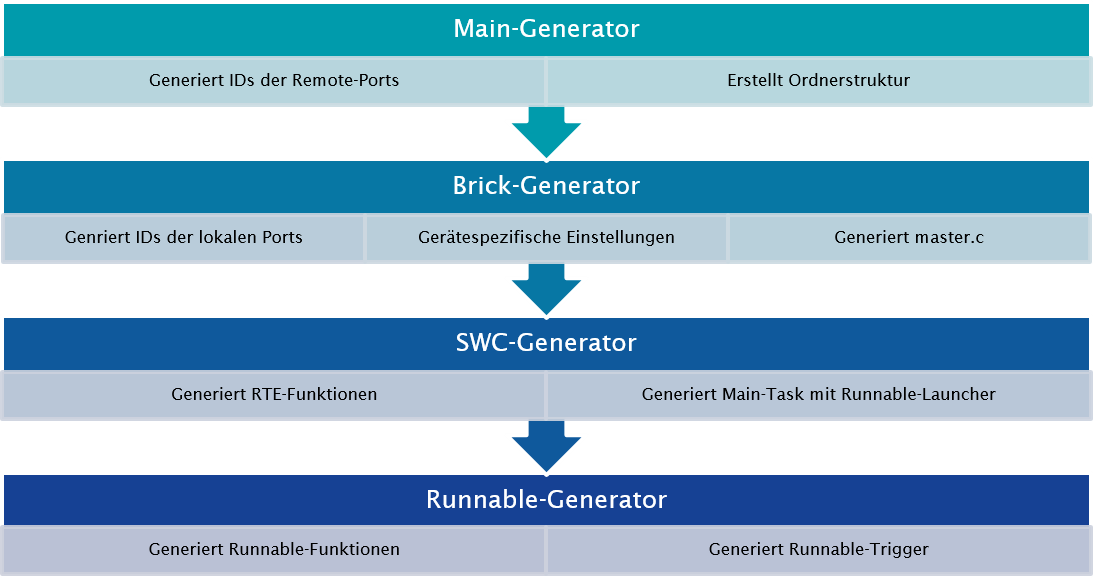
\includegraphics[width=\textwidth]{Dokumente/generator_architektur}
	\caption{Hierarchische Architektur des Generators}
	\label{fig:hardwareaufbau}
\end{figure}

Die Architektur folgt der hierarchischen Struktur des EMF Modells in groben Zügen, wie in Abbildung \ref{fig:hardwareaufbau} zu sehen ist.

Diese Architektur erlaubt es, Informationen leicht in tiefere Ebenen des Generators weiterzugeben. Außerdem erlaubt es die Architektur, atomare Kleinst-Generatoren nachträglich einzufügen. Dritte könnten beispielsweise eine neue Art von Software-Ports einfügen, indem sie die Generator-Klasse innerhalb der Klasse \texttt{SoftwarePortGenerator} einfügen. Weiteres Wissen über die Architektur des Generators sind nicht nötig.

Die Generatoren gliedern sich generell in die 3 (optionalen) Phasen \textit{prepare}, \textit{process} und \textit{persist}.
\begin{itemize}
\item \textbf{prepare}: Kontextinformationen für Unter-Generatoren werden gesammelt und Untergeneratoren werden aufgerufen.
\item \textbf{process}: Informationen für aktuellen Generator werden gesammelt, Template-Operationen werden vorbereitet.
\item \textbf{persist}: Templates werden geladen und generierte Dateien geschrieben.
\end{itemize}

Die vordefinierte Struktur erlaubt die einfache Erweiterung des Generators. Zusätzliche Funktionalität kann, je nach Bedarf, vor oder nach einer der 3 Phasen eingehängt werden.

\subsection{Templates}
Innerhalb der Generatoren, werden die benötigten Informationen aus dem Metamodell zusammengetragen. Anschließend wird ein Template aus dem Resourcen-Ordner geladen. Templates sind Vorlagen für generierte Dateien. Diese sind unabhängig von der Programmiersprache, da meistens nur einfache Textersetzungen durchgeführt werden. Im Vergleich zu den bekannten \texttt{defines} erlauben Templates komplexere Ersetzungen, da der Code zur Ersetzung völlig anpassbar ist. Zusätzlich ist diese Variante nicht abhängig von der Programmiersprache und deshalb universell einsetzbar.
Templates können außerdem ohne jegliche Java-Kenntnisse editiert werden.

\begin{lstlisting}[frame=single, language=c, label=lst:task_template, caption=Template für Task-Definition]  
TASK <TASK_NAME>
{
	AUTOSTART = <AUTOSTART>;
	PRIORITY = <PRIORITY>;	
	<EVENT>
};
\end{lstlisting}

In Abbildung \ref{lst:task_template} ist zu erkennen, dass Templates den generierten Dateien sehr ähnlich sind. Einzig die Variablen in spitzen Klammern werden ersetzt. Das kann in trivialer Form geschehen, wie zum Beispiel bei \texttt{<AUTOSTART>} oder \texttt{<PRIORITY>}. Hier werden die Variablen einfach durch die berechneten Werte ersetzt. Im Fall von \texttt{<EVENT>} jedoch, wird eine benutzerdefinierte Logik eingesetzt. So kann die Variable gleich mehrfach ersetzt werden, um mehrere Events zu registrieren.


\section{Generierte Struktur}

Der Generator generiert für jeden Brick einen eigenen Ordner Namens Brick\textunderscore \texttt{BrickName}. Diese enthalten folgende Dateien. Die Dateien in den Brick-Ordnern dürfen nicht vom User bearbeitet werden.

\begin{itemize}
\item \textbf{master.oil:} Definition aller benötigter Tasks, Events, Alarme, etc.
\item \textbf{master.c} Initialisierung der Hardware, Definition der Events/Tasks/etc., Initialisierung der Port-Arrays, Verarbeitung von Bluetooth-Daten.
\item \textbf{SWC\textunderscore <SWC-Name>.c} Enthält alle, für die SWC benötigten RTE-Funktionen.
\item \textbf{defines.h} Enthält Gerätespezifische Defines zur Konfiguration der Handler.
\end{itemize}

Für jeden Brick sowie für die Runnables werden vom Generator Ordner angelegt. Der Ordner \texttt{Runnables} enthält einen Stub für jedes Runnable. Diese müssen dann vom User implementiert werden.

Parallel zu diesen Ordnern, muss vom User der Ordner \texttt{BSW} abgelegt werden, der die Basissoftware enthält.

Außerdem müssen Makefiles vom User angelegt werden, da die Zeit nicht mehr erlaubte, diese zu generieren.
